
	%pi-calc commands
			
			
	\newcommand{\picalc}{%
		\texorpdfstring{$\pi$}{pi}-calculus}
	% \newcommand{\HUGE}{\fontsize{43}{54}\selectfont}
	% \newcommand{\PICALC}{%
	% 	\texorpdfstring{{\Huge{$\pi$}}}{pi}-Calculus\ %
	% }
	\newcommand{\exports}[1]{%
	\ensuremath{({#1})}%
	}
	\newcommand{\Picalc}{%
		\texorpdfstring{$\pi$}{pi}-Calculus}
	
	\newcommand{\send}[2]{%
	 	\ensuremath{{#1}!\langle{#2}\rangle}%
	}
	\newcommand{\sends}[2]{%
	 	\ensuremath{{#1}!{#2}}%
	}
	\newcommand{\ssend}[2]{%
	 	\ensuremath{{#1}!\langle{#2}\rangle.}%
	}
	\newcommand{\receives}[2]{%
	 	\ensuremath{{#1}?{#2}}%
	}
	\newcommand{\receive}[2]{%
	 	\ensuremath{{#1}?({#2}).}%
	}
	\newcommand{\receivenodot}[2]{%
	 	\ensuremath{{#1}?({#2})}%
	}
	\newcommand{\new}[1]{%
	 	\ensuremath{\text{new}({#1}).}%
	}
	\newcommand{\pif}[1]{%
		\ensuremath{\text{if } {#1}}%
	}
	\newcommand{\pthen}{%
		\ensuremath{\text{ then }}%
	}
	\newcommand{\pelse}{%
		 \ensuremath{\text{ else }}%
	}
	\newcommand{\comp}{%
		\ensuremath{\ |\ }%
	}
	\newcommand{\rec}[1]{%
		\ensuremath{\text{rec }{#1}.}%
	}
	\newcommand{\defequals}{%
	 \ensuremath{\overset{\tiny{def}}{=}}%
	}
	\newcommand{\encode}[1]{%
	 \ensuremath{\llbracket{#1}\rrbracket}%
	}
	\newcommand{\subst}[2]{%
	 \ensuremath{\llbracket{#1}/{#2}\rrbracket}%
	}
	\newcommand{\pdef}{\ensuremath{\Leftarrow}\ }
	\newcommand{\sys}[1]{\ensuremath{\mathbb{#1}}}
	\newcommand{\sequiv}{\ensuremath{\equiv}}
	\newcommand{\pred}{\ensuremath{\longrightarrow}}
	\newcommand{\evolves}[1]{\ensuremath{\overset{{#1}}{\longrightarrow}}}
	
	\newcommand{\preds}{\ensuremath{\cdotp\!\cdotp\!\cdotp\!\longrightarrow}}
	%end pi-calc commands
\documentclass[12pt,twoside]{reedthesis}
\usepackage{graphicx,latexsym} 
\usepackage{amssymb,amsthm,amsmath}
\usepackage{longtable,booktabs,setspace} 
\usepackage{url}
\usepackage{float}
\usepackage{natbib}
\usepackage{multirow}
\usepackage{datetime}
% \usepackage{a0size} used for a really big pi symbol - disabled

\usepackage[palatino]{quotchapwc} %figure out where to stick \thispagestyle{empty}%
\renewcommand\chapterheadstartvskip{\vspace*{-5\baselineskip}}
\usepackage[calcwidth]{titlesec}

\setlength{\parskip}{0pt}
\usepackage[bookmarks, colorlinks=true, linkcolor=black, citecolor= black, pdftitle={The $pi$-calculus}, pdfauthor={William Henderson}]{hyperref}

\begin{document}
	  \pagestyle{empty}
		%%%%%%%%%%%%%%%%%%%%%%%%%%%%%%%%%%%%%%%%%%%%%%%%%%%%%%%%%%%%%%%%%
		\null\vfil
		\centering \textbf{The Phone}:
		\[
			Mobile(talk, switch) \pdef \ssend{talk}{} Mobile\langle talk,switch\rangle + \receive{switch}{t,s} Mobile\langle t,s\rangle
		\]\\[20pt]
		
		\centering \textbf{The Tower}:
		\begin{align*}
			ActiveT(talk,switch,gain,lose) \pdef & \receive{talk}{}ActiveT\langle talk,switch,gain,lose\rangle \\  
			 & +\receive{lose}{t,s}\ssend{switch}{t,s}IdleT\langle gain, lose\rangle\\
			IdleT(gain,lose) \pdef & \receive{gain}{t,s}ActiveT\langle t,s,gain,lose\rangle\\
		\end{align*}\\[20pt]
		
		\centering \textbf{The Server}:
		\begin{align*}
			Server_1 \pdef \ssend{lose_1}{talk_2,switch_2} \ssend{gain_2}{talk_2,switch_2} Server_2\\
			Server_2 \pdef \ssend{lose_2}{talk_1,switch_1} \ssend{gain_1}{talk_1,switch_1} Server_1
		\end{align*}
		\newpage
		%%%%%%%%%%%%%%%%%%%%%%%%%%%%%%%%%%%%%%%%%%%%%%%%%%%%%%%%%%%%%%%%%
		\null\vfil
		\begin{figure}[H]
		\centering
		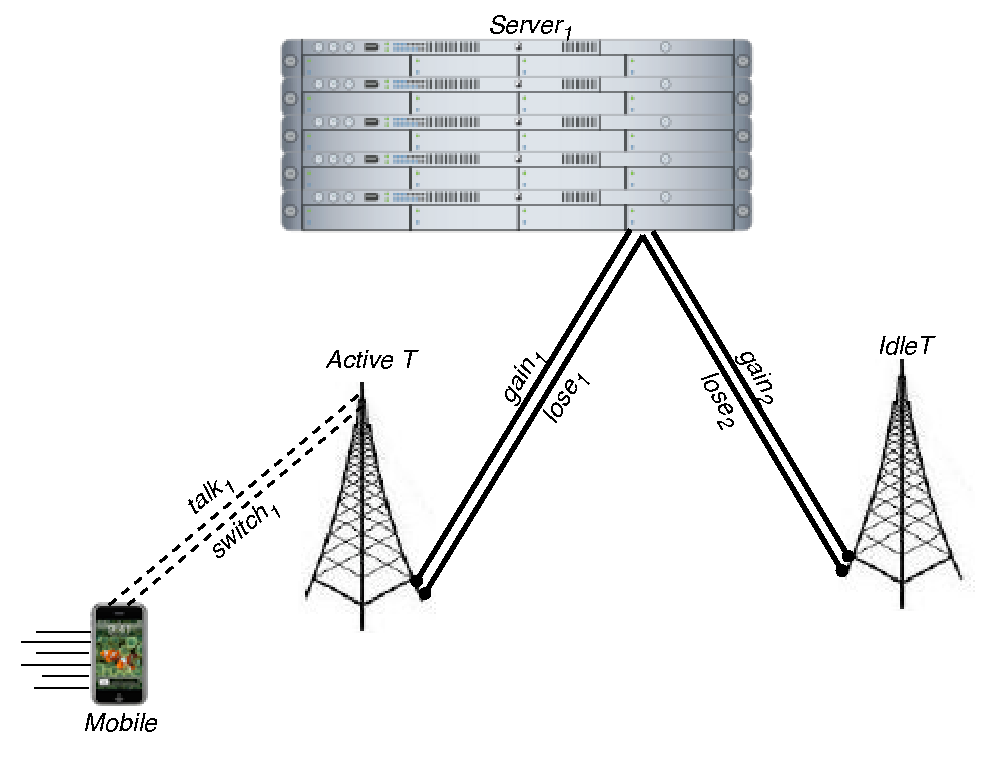
\includegraphics[scale=0.7]{figures/cell_network_pi.pdf} % requires the graphicx package
		\caption{\emph{Simplified mobile phone network in the \picalc}}
		\label{fig_cell_network_pi}
		\end{figure}
		\newpage
		%%%%%%%%%%%%%%%%%%%%%%%%%%%%%%%%%%%%%%%%%%%%%%%%%%%%%%%%%%%%%%%%%
		\null\vfil
	  		
		\begin{insettable}
		\begin{center}
		\begin{tabular}{r l l}
		\multicolumn{3}{c}{\emph{Process terms}}\\
		$R :=$  &$R_1 \comp R_2$ & Composition\\
		&\send{n}{\tuple{V}} & Send\\
		&$\receive{n}{\tuple{X}} R$ & Receive\\
		&$\new{n}R$ & Restriction\\
		&$\pif{v_1 = v_2}\pthen R_1 \pelse R_2$ & Matching\\
		&$\rec{p} R$ & Recursion\\
		&\pstop & Termination\\
		&\\
		
		\multicolumn{3}{c}{\emph{System}} \\
		& $\new{c_1,...,c_n} R_1 \comp...\comp R_m$ & $n, m >= 0$\\
		\end{tabular}
		\caption{\emph{Terms in the asynchronous \picalc}}\label{apicalcterms}
		\end{center}
		\end{insettable}
		\newpage
		%%%%%%%%%%%%%%%%%%%%%%%%%%%%%%%%%%%%%%%%%%%%%%%%%%%%%%%%%%%%%%%%%
	  	\null\vfil
		
		\begin{align*}
			P{'}(a) \pdef \receive{a}{x}(\new{n'}(\send{n'}{} \comp \send{c}{}))
		\end{align*}
		\centering is $\alpha$-equivalent to
		\begin{align*}
			P(a) \pdef \receive{a}{x}(\new{n}(\send{n}{} \comp \send{x}{}))
		\end{align*}
		\\[20pt]
		\centering (which terms are bound?)
		
		\newpage
		%%%%%%%%%%%%%%%%%%%%%%%%%%%%%%%%%%%%%%%%%%%%%%%%%%%%%%%%%%%%%%%%%
		\null\vfil
	  
		\begin{definition}{Structural Equivalence}
			Structural Equivalence, denoted $\sequiv$ is the smallest contextual equivalence relation that satisfies the following axioms:
			\begin{align*}
				P \comp Q\ &\  \sequiv\  Q \comp P && \text{\tiny{(S-COMP-COMM)}}\\
			 	(P \comp Q) \comp R\ &\ \sequiv\ P \comp (Q \comp R) && \text{\tiny{(S-COMP-ASSOC)}}\\
				P \comp \pstop\ &\ \sequiv\ P && \text{\tiny{(S-COMP-ID)}}\\
				\new{c} \pstop\ &\ \sequiv\ \pstop && \text{\tiny{(S-REST-ID)}}\\
				\new{c}\new{d} P \ &\ \sequiv\ \new{d}\new{c} P && \text{\tiny{(S-REST-COMM)}}\\
				\new{c}(P \comp Q)\ &\ \sequiv\  P \comp \new{c}Q\text{, if } c\not\in \mbox{fi}(P) && \text{\tiny{(S-REST-COMP)}}
			\end{align*}
		\end{definition}\index{structural equivalence}
		\newpage
		%%%%%%%%%%%%%%%%%%%%%%%%%%%%%%%%%%%%%%%%%%%%%%%%%%%%%%%%%%%%%%%%%
	  	\null\vfil
	
		\begin{definition}{Reduction}
			The \emph{reduction relation} \pred\ is the smallest contextual relation that satisfies the following rules:
			\begin{center}\begin{tabular}{rll}
				$\send{c}{\tuple{V}} \comp \receive{c}{\tuple{X}}R$\ &\  $\pred\  R\subst{\tuple{V}}{\tuple{X}}$ & \tiny{(R-COMM)}\\
				$\rec{p}R$\ &\  $\pred\  R\subst{\rec{p}R}{p}$ & \tiny{(R-REP)}\\
				$\pif{v = v}\pthen P \pelse Q$\ &\ $\pred\ P$ & \tiny{(R-EQ)}\\
				$\pif{v_1 = v_2}\pthen P \pelse Q$\ &\ $\pred\ Q$ \ \ (where $v_1\neq v_2$)& \tiny{(R-NEQ)}\\
				\multicolumn{2}{c}{\hspace{4.5em}$\underline{P\sequiv P', P \pred Q, Q\sequiv Q'}$} & \multirow{2}{*}{\tiny{(R-STRUC)}}\\
				\multicolumn{2}{c}{\hspace{4.5em}$P'\pred Q'$}
			\end{tabular}\end{center}
			We use the notation $P\preds Q$ when an arbitrary number of these rules have been applied in reducing $P$ to $Q$.
		\end{definition}\index{reduction}
		
		\newpage
		%%%%%%%%%%%%%%%%%%%%%%%%%%%%%%%%%%%%%%%%%%%%%%%%%%%%%%%%%%%%%%%%%
		\null\vfil
	  
		\begin{definition}{Action}\label{apiactionrules}
			The \emph{action relation} \evolves{} is the smallest relation between processes that satisfy the following rules:
			\begin{center}\begin{tabular}{rllll}
		 		$\receive{c}{\tuple{X}}R$ & \evolves{\receives{c}{\tuple{V}}} & R\subst{\tuple{V}}{\tuple{X}} & & \tiny{(A-IN)}\\
				$\send{c}{\tuple{V}}$ & \evolves{\sends{c}{\tuple{V}}} & $\pstop$ & & \tiny{(A-OUT)}\\
				$\rec{x}R$ & \evolves{\tau} & $R\subst{\rec{x}R}{x}$ & & \tiny{(A-REP)}\\
				$\pif{v=v} \pthen P \pelse Q$ & \evolves{\tau} & $P$ & & \tiny{(A-EQ)}\\[10pt]
				$\pif{v_1=v_2} \pthen P \pelse Q$ & \evolves{\tau} & $Q$ & $v_1 \neq v_2$ & \tiny{(A-NEQ)}\\[10pt]

				\multicolumn{3}{c}{$\underline{P \evolves{\alpha} P'}$} & \multirow{2}{*}{\footnotesize{$\textstyle bn(\alpha) \cap fn(Q) = \emptyset$ }} & \multirow{2}{*}{\tiny{(A-COMP)}}\\
				\multicolumn{3}{c}{$P\comp Q \evolves{\alpha} P'\comp Q$}\\[10pt]

				\multicolumn{3}{c}{$\underline{P \evolves{\alpha} P'}$} & \multirow{2}{*}{\footnotesize{$\textstyle b \not \in n(\alpha)$ }} & \multirow{2}{*}{\tiny{(A-REST)}}\\
				\multicolumn{3}{c}{$\new{b} P \evolves{\alpha} \new{b} P'$}\\[10pt]

				\multicolumn{3}{c}{$\underline{P\evolves{\exports{\tuple{B}}\sends{c}{\tuple{V}}} P'}$} & \multirow{2}{*}{\footnotesize{$n \neq c, n \text{ is in } \tuple{V}$ }}& \multirow{2}{*}{\tiny{(A-OPEN)}}\\
				\multicolumn{3}{c}{$\new{n}P \evolves{\exports{n,\tuple{B}}\sends{c}{\tuple{V}}} P'$}\\[10pt]

				\multicolumn{3}{c}{$\underline{P\evolves{\receives{c}{\tuple{V}}} P',\ Q \evolves{\exports{\tuple{B}}\sends{c}{\tuple{V}}} Q'}$} & \multirow{2}{*}{\footnotesize{$\textstyle \exports{\tuple{B}}\cap fn(P) = \emptyset$ }} & \multirow{2}{*}{\tiny{(A-COMM)}}\\
				\multicolumn{3}{c}{$P\comp Q \evolves{\tau} \new{\tuple{B}}(P'\comp Q')$}\\[10pt]
			\end{tabular}\end{center}
		\end{definition}
		\newpage
		%%%%%%%%%%%%%%%%%%%%%%%%%%%%%%%%%%%%%%%%%%%%%%%%%%%%%%%%%%%%%%%%%
		\null\vfil
	  
		\begin{insettable}
		\begin{center}
		\begin{tabular}{r l l}
		\multicolumn{3}{c}{\emph{Action Prefixes}}\\
		$\pi :=$  & $\send{n}{\tuple{V}}$ & Send\\
		&$\receivenodot{n}{\tuple{X}}$ & Receive\\

		&\\

		\multicolumn{3}{c}{\emph{Process terms}}\\
		$R :=$ & $\displaystyle\sum_{i} \pi_i.R_i$ &\multirow{2}{*}{Summation}\\[20pt]
		&$R_1 \comp R_2$ & Composition\\
		&$\new{n}R$ & Restriction\\
		&$\pif{v_1 = v_2}\pthen R_1 \pelse R_2$ & Matching\\
		&$\rec{x} R$ & Recursion\\
		&\pstop & Termination\\
		&\\
		\end{tabular}
		\caption{\emph{Terms in the synchronous \picalc}}\label{spicalcterms}
		\end{center}
		\end{insettable}
		\newpage
		%%%%%%%%%%%%%%%%%%%%%%%%%%%%%%%%%%%%%%%%%%%%%%%%%%%%%%%%%%%%%%%%%
		\null\vfil
	  
		\begin{quote}
			\textbf{Lemma 4.1} \emph{Let P be a process of the asynchronous \picalc.  Assume that P can make two transitions $P \evolves{\alpha_s} Q$ and $P \evolves{\alpha_r} Q'$, where $\alpha_s$ is a send action while $\alpha_r$ is a receive action.  Then there exists a process R such that $Q \evolves{\alpha_r} R$ and $Q' \evolves{\alpha_s} R$.}
		\end{quote}
		\centering Consider, for example:
		
		\begin{align*}
			P_0\comp P_1 \pdef \ssend{c_0}{} \send{o}{c_0} + \receive{c_1}{} \send{o}{c_1} \comp \ssend{c_1}{} \send{o}{c_1} + \receive{c_0}{} \send{o}{c_0}
		\end{align*}
		
		\newpage
		%%%%%%%%%%%%%%%%%%%%%%%%%%%%%%%%%%%%%%%%%%%%%%%%%%%%%%%%%%%%%%%%%
		\null\vfil
	  
		\centering Palamidessi uses the separation results to construct two criteria for encodings:\\[20pt]

		\textbf{Uniformity}:
		\begin{align*}
			\encode{\sigma(P)} &= \sigma(\encode{P})\\
			\encode{P\comp Q} &= \encode{P} \comp \encode{Q}
		\end{align*}
		
		\textbf{Reasonability}:
		\begin{quote}
			\emph{the capability of a language to distinguish between two processes when their actions  given channel differ.}
		\end{quote}
		
		\newpage
		%%%%%%%%%%%%%%%%%%%%%%%%%%%%%%%%%%%%%%%%%%%%%%%%%%%%%%%%%%%%%%%%%
	  	\null\vfil
	
		\centering \textbf{Summation}:
		\[
			\encode{\displaystyle\sum_{i} \pi_i.R_i} \defequals \new{l}(\send{l}{\ptrue} \comp \displaystyle\prod_{i}\encode{\pi_i.R_i}_l)
		\]\\[20pt]
		
		\centering \textbf{Sending}:
		\begin{equation*}\begin{split}
			\encode{\ssend{c}{\tuple{V}}P}_r \defequals & \new{ack}(\send{c}{r,ack,\tuple{V}} \comp \receive{ack}{x} \pif{x=\ptrue} \pthen \encode{P} \\
			&\pelse (\pif{x=\pretry} \pthen \send{c}{r,ack,\tuple{V}} \pelse \pstop))
		\end{split}\end{equation*}\\[20pt]
		
		\centering \textbf{Receiving}:
		\begin{equation*}\begin{split}
			\encode{\receive{c}{\tuple{X}}P}_l \defequals & \rec{q}\receive{c}{r,ack,\tuple{X}} (l,r)?d\mbox{\emph{-}}lock.\encode{P}
		\end{split}\end{equation*}\\[20pt]
		
		\centering $\mathbf{(l,r)?d\mbox{\emph{-}}lock.P}$ \textbf{means}:
		\begin{equation*}\begin{split}
			\receive{l}{x}(&\pif{x=\ptrue}\\
			&\pthen \receive{r}{y} (\pif {y=\ptrue}\\
			&\ \ \ \ \ \ \pthen \send{l}{\pfalse} \comp \send{r}{\pfalse} \comp \send{ack}{\ptrue} \comp P\\
			&\ \ \ \ \ \ \pelse \send{l}{\ptrue} \comp \send{r}{\pfalse} \comp \send{ack}{\pfalse} \comp q)\\
			&\pelse\send{l}{\pfalse} \comp \send{ack}{\pretry})\\
		\end{split}\end{equation*}
		
		\newpage
		%%%%%%%%%%%%%%%%%%%%%%%%%%%%%%%%%%%%%%%%%%%%%%%%%%%%%%%%%%%%%%%%%
		\null\vfil
	  
		\centering \textbf{Summation}:
		\[
			\encode{\displaystyle\sum_{i} \pi_i.R_i}^d \defequals \receive{d}{n}(\send{d}{n+1} \comp \new{l}(\send{l}{\ptrue} \comp \displaystyle\prod_{i}\encode{\pi_i.R_i}^d_{n,l}))
		\]\\[20pt]
		
		\centering \textbf{Sending}:
		\begin{equation*}\begin{split}
			\encode{\ssend{c}{\tuple{V}}P}^d_{n,l} \defequals & \new{ack}(\send{c}{n,l,ack,\tuple{V}} \comp \receive{ack}{x} \pif{x=\ptrue} \pthen \encode{P}^d \\
			&\pelse (\pif{x=\pretry} \pthen \send{c}{n,l,ack,\tuple{V}} \pelse \pstop))
		\end{split}\end{equation*}\\[20pt]
		
		\centering \textbf{Receiving}:
		\begin{equation*}\begin{split}
			\encode{\receive{c}{\tuple{X}}P}^d_{n,l} \defequals & \rec{q}(\receive{c}{m,r,ack,\tuple{X}}(\\
			&\pif{n=m} \pthen (\send{ack}{\pretry}\comp q) \pelse(\\
			&\pif{n<m} \pthen (l,r)?d\mbox{\emph{-}}lock.\encode{P}^d \pelse (r,l)?rd\mbox{\emph{-}}lock.\encode{P}^d)))\\
		\end{split}\end{equation*}\\[20pt]
		
		\begin{table}[ht]
		\hspace{-2.5cm}	
		\begin{minipage}[b]{.5\textwidth}
		\centering $\mathbf{(l,r)?d\mbox{\emph{-}}lock.P}$ \textbf{means}:
		\begin{equation*}\begin{split}
			\receive{l}{x}(&\pif{x=\ptrue}\\
			&\pthen \receive{r}{y} (\pif {y=\ptrue}\\
			&\ \ \ \ \ \ \pthen \send{l}{\pfalse} \comp \send{r}{\pfalse} \comp \send{ack}{\ptrue} \comp P\\
			&\ \ \ \ \ \ \pelse \send{l}{\ptrue} \comp \send{r}{\pfalse} \comp \send{ack}{\pfalse} \comp q)\\
			&\pelse\send{l}{\pfalse} \comp \send{ack}{\pretry})\\
		\end{split}\end{equation*}
	\end{minipage}
	\hspace{2.5cm}
	\begin{minipage}[b]{.5\textwidth}	
		\centering $\mathbf{(r,l)?rd\mbox{\emph{-}}lock.P}$ \textbf{means}:
		\begin{equation*}\begin{split}
			\receive{r}{x}(&\pif{x=\ptrue}\\
			&\pthen \receive{l}{y} (\pif {y=\ptrue}\\
			&\ \ \ \ \ \ \pthen \send{l}{\pfalse} \comp \send{r}{\pfalse} \comp \send{ack}{\ptrue} \comp P\\
			&\ \ \ \ \ \ \pelse \send{l}{\pfalse} \comp \send{r}{\ptrue} \comp \send{ack}{\pretry})\\
			&\pelse\send{r}{\pfalse} \comp \send{ack}{\pfalse}\comp q)\\
		\end{split}\end{equation*}
	\end{minipage}
	\end{table}
\end{document}